\section{manifold\_\-fullsim.cc File Reference}
\label{manifold__fullsim_8cc}\index{manifold\_\-fullsim.cc@{manifold\_\-fullsim.cc}}
{\tt \#include \char`\"{}mesh.h\char`\"{}}\par
{\tt \#include \char`\"{}../../zesto/zesto-uncore.h\char`\"{}}\par
{\tt \#include \char`\"{}../../util/config\_\-params.h\char`\"{}}\par


Include dependency graph for manifold\_\-fullsim.cc:\nopagebreak
\begin{figure}[H]
\begin{center}
\leavevmode
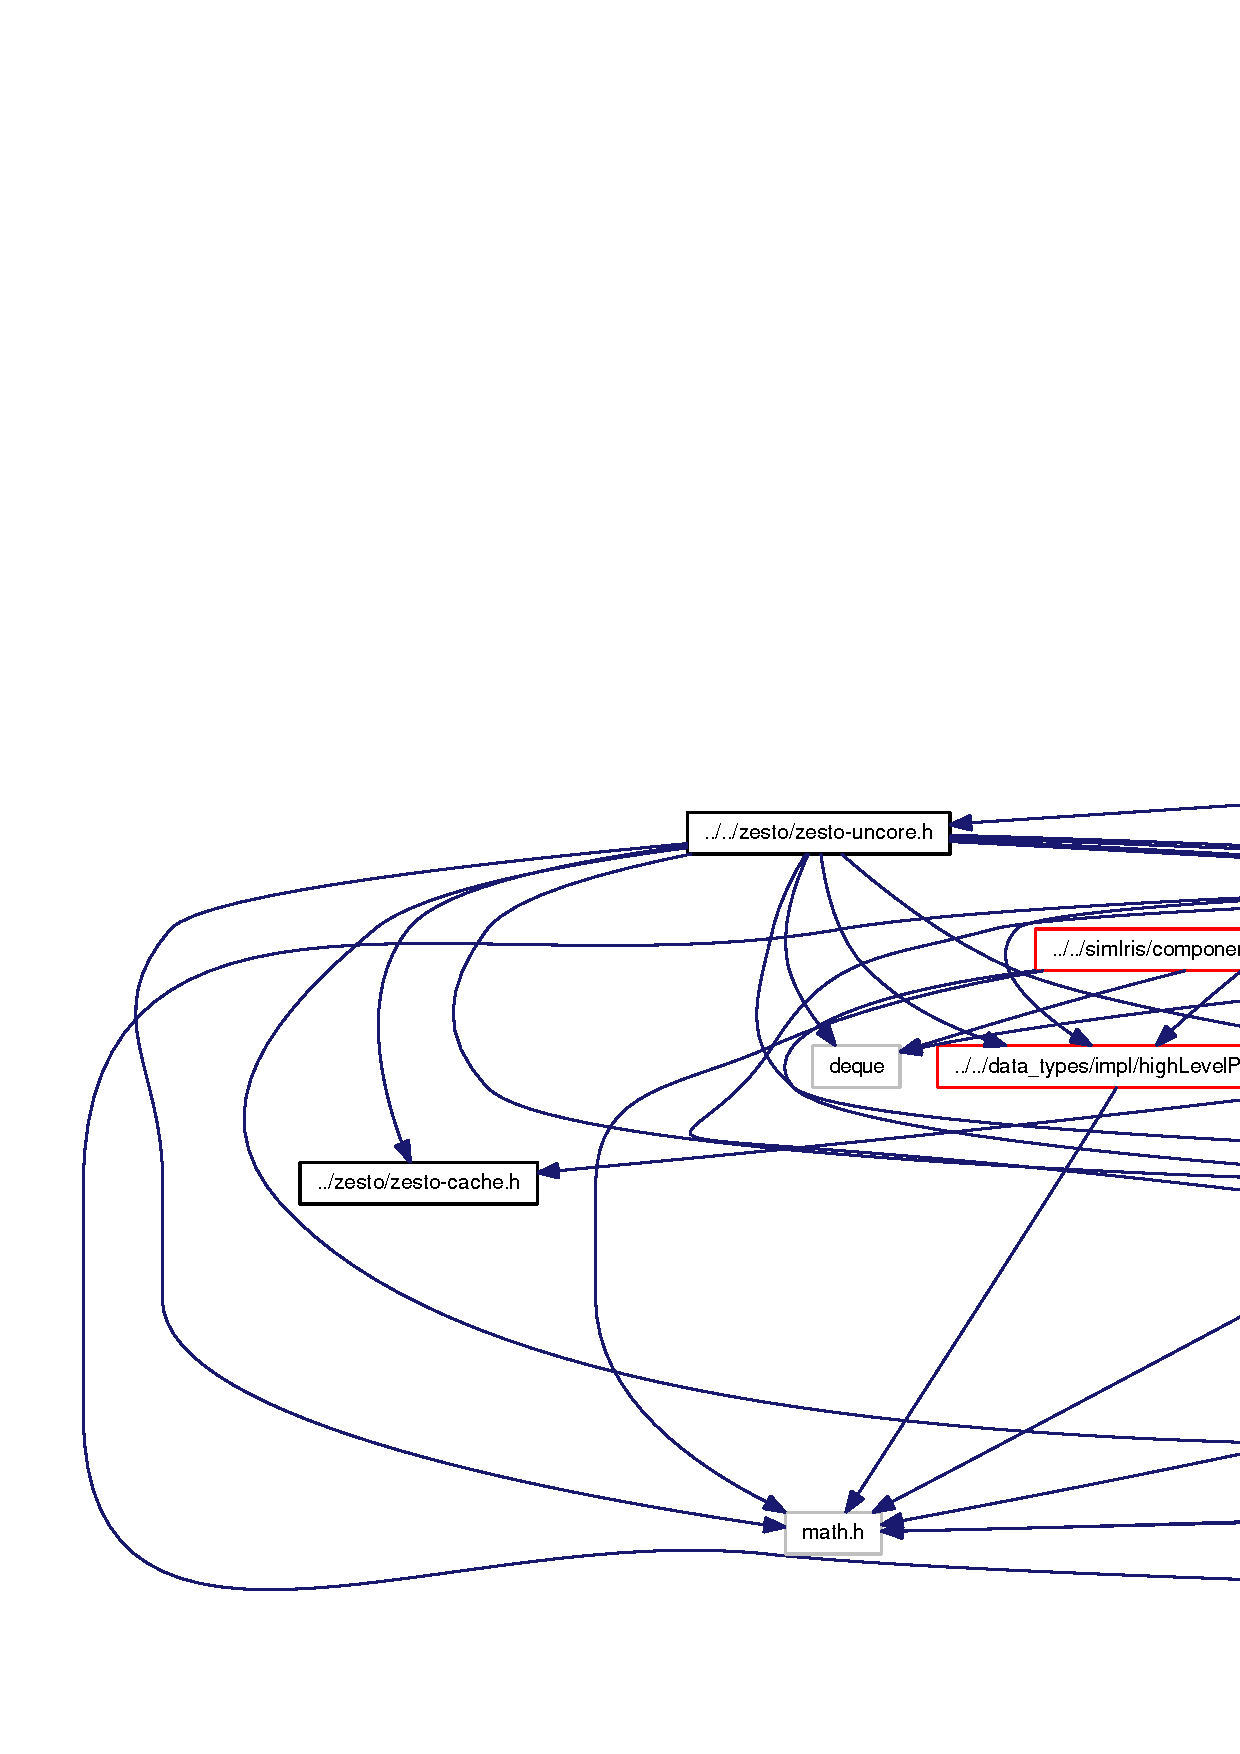
\includegraphics[width=420pt]{manifold__fullsim_8cc__incl}
\end{center}
\end{figure}
\subsection*{Functions}
\begin{CompactItemize}
\item 
void {\bf print\_\-state\_\-at\_\-deadlock} (void)
\item 
static void {\bf signal\_\-sim\_\-stats} (int sigtype)
\item 
static void {\bf signal\_\-exit\_\-now} (int sigtype)
\item 
static int {\bf orphan\_\-fn} (int i, int argc, char $\ast$$\ast$argv)
\item 
static void {\bf banner} (FILE $\ast$fd, int argc, char $\ast$$\ast$argv)
\item 
static void {\bf usage} (FILE $\ast$fd, int argc, char $\ast$$\ast$argv)
\item 
void {\bf sim\_\-print\_\-stats} (FILE $\ast$fd)
\item 
static void {\bf exit\_\-now} (int {\bf exit\_\-code})
\item 
unsigned int {\bf iris\_\-process\_\-options} (int argc, char $\ast$argv[$\,$])
\item 
void {\bf iris\_\-init} ()
\item 
int {\bf main} (int argc, char $\ast$argv[$\,$])
\end{CompactItemize}
\subsection*{Variables}
\begin{CompactItemize}
\item 
string {\bf data}
\item 
string {\bf word}
\item 
unsigned int {\bf cores\_\-per\_\-node} = 1
\item 
{\bf Mesh} $\ast$ {\bf mesh}
\item 
char $\ast$ {\bf s}
\item 
int {\bf exit\_\-code}
\item 
time\_\-t {\bf sim\_\-start\_\-time}
\item 
time\_\-t {\bf sim\_\-end\_\-time}
\item 
int {\bf sim\_\-elapsed\_\-time}
\item 
int {\bf sim\_\-swap\_\-bytes}
\item 
int {\bf sim\_\-swap\_\-words}
\item 
int {\bf sim\_\-exit\_\-now} = FALSE
\item 
jmp\_\-buf {\bf sim\_\-exit\_\-buf}
\item 
int {\bf sim\_\-dump\_\-stats} = FALSE
\item 
struct {\bf opt\_\-odb\_\-t} $\ast$ {\bf sim\_\-odb}
\item 
struct {\bf stat\_\-sdb\_\-t} $\ast$ {\bf sim\_\-sdb}
\item 
char $\ast$ {\bf sim\_\-simout} = NULL
\item 
char $\ast$ {\bf sim\_\-progout} = NULL
\item 
FILE $\ast$ {\bf sim\_\-progfd} = NULL
\item 
static int {\bf exec\_\-index} = -1
\item 
bool {\bf help\_\-me}
\item 
int {\bf rand\_\-seed}
\item 
bool {\bf init\_\-quit}
\item 
int {\bf nice\_\-priority}
\item 
static int {\bf running} = FALSE
\end{CompactItemize}


\subsection{Function Documentation}
\index{manifold\_\-fullsim.cc@{manifold\_\-fullsim.cc}!banner@{banner}}
\index{banner@{banner}!manifold_fullsim.cc@{manifold\_\-fullsim.cc}}
\subsubsection[{banner}]{\setlength{\rightskip}{0pt plus 5cm}static void banner (FILE $\ast$ {\em fd}, \/  int {\em argc}, \/  char $\ast$$\ast$ {\em argv})\hspace{0.3cm}{\tt  [static]}}\label{manifold__fullsim_8cc_bb4b863ca4fbb167c2f78c8ad25f16cd}




Definition at line 128 of file manifold\_\-fullsim.cc.

References s, VER\_\-MAJOR, VER\_\-MINOR, and VER\_\-UPDATE.

Referenced by main().

Here is the caller graph for this function:\nopagebreak
\begin{figure}[H]
\begin{center}
\leavevmode
\includegraphics[width=82pt]{manifold__fullsim_8cc_bb4b863ca4fbb167c2f78c8ad25f16cd_icgraph}
\end{center}
\end{figure}
\index{manifold\_\-fullsim.cc@{manifold\_\-fullsim.cc}!exit\_\-now@{exit\_\-now}}
\index{exit\_\-now@{exit\_\-now}!manifold_fullsim.cc@{manifold\_\-fullsim.cc}}
\subsubsection[{exit\_\-now}]{\setlength{\rightskip}{0pt plus 5cm}static void exit\_\-now (int {\em exit\_\-code})\hspace{0.3cm}{\tt  [static]}}\label{manifold__fullsim_8cc_8cf40713cf8239d39ed7d0967eec7cf4}




Definition at line 237 of file manifold\_\-fullsim.cc.

References sim\_\-print\_\-stats(), and sim\_\-uninit().

Referenced by main().

Here is the caller graph for this function:\nopagebreak
\begin{figure}[H]
\begin{center}
\leavevmode
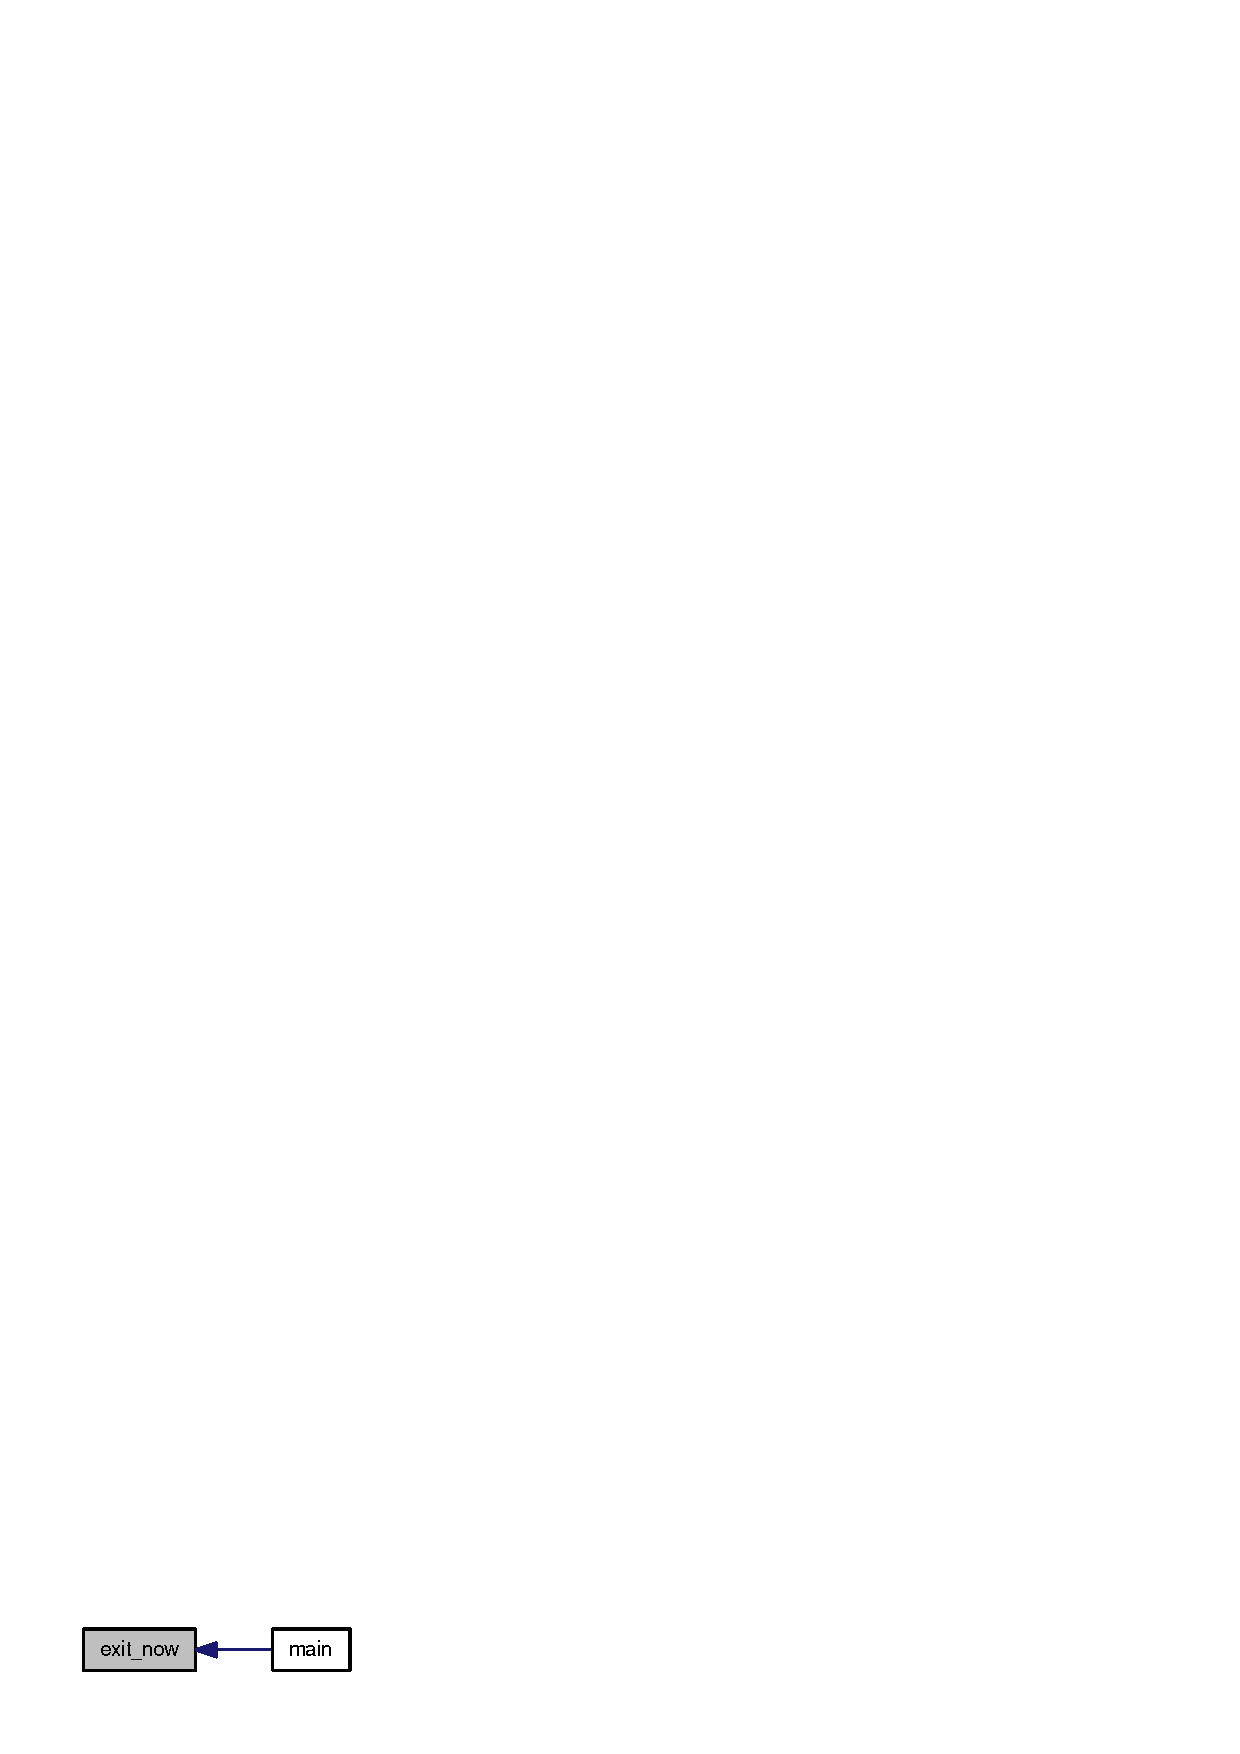
\includegraphics[width=86pt]{manifold__fullsim_8cc_8cf40713cf8239d39ed7d0967eec7cf4_icgraph}
\end{center}
\end{figure}
\index{manifold\_\-fullsim.cc@{manifold\_\-fullsim.cc}!iris\_\-init@{iris\_\-init}}
\index{iris\_\-init@{iris\_\-init}!manifold_fullsim.cc@{manifold\_\-fullsim.cc}}
\subsubsection[{iris\_\-init}]{\setlength{\rightskip}{0pt plus 5cm}void iris\_\-init ()}\label{manifold__fullsim_8cc_9ceb71c1e1d68963b68464d4bd3aed81}




Definition at line 422 of file manifold\_\-fullsim.cc.

References buffer\_\-size, Mesh::connect\_\-interface\_\-processor(), Mesh::connect\_\-interface\_\-routers(), Mesh::connect\_\-routers(), credits, grid\_\-size, Mesh::init(), Mesh::interfaces, Mesh::link\_\-a, Mesh::link\_\-b, links, max\_\-sim\_\-time, Mesh::max\_\-sim\_\-time, mc\_\-positions, no\_\-nodes, ports, print\_\-setup, Mesh::processors, Mesh::routers, Mesh::setup(), uncores, and vcs.

Referenced by main().

Here is the caller graph for this function:\nopagebreak
\begin{figure}[H]
\begin{center}
\leavevmode
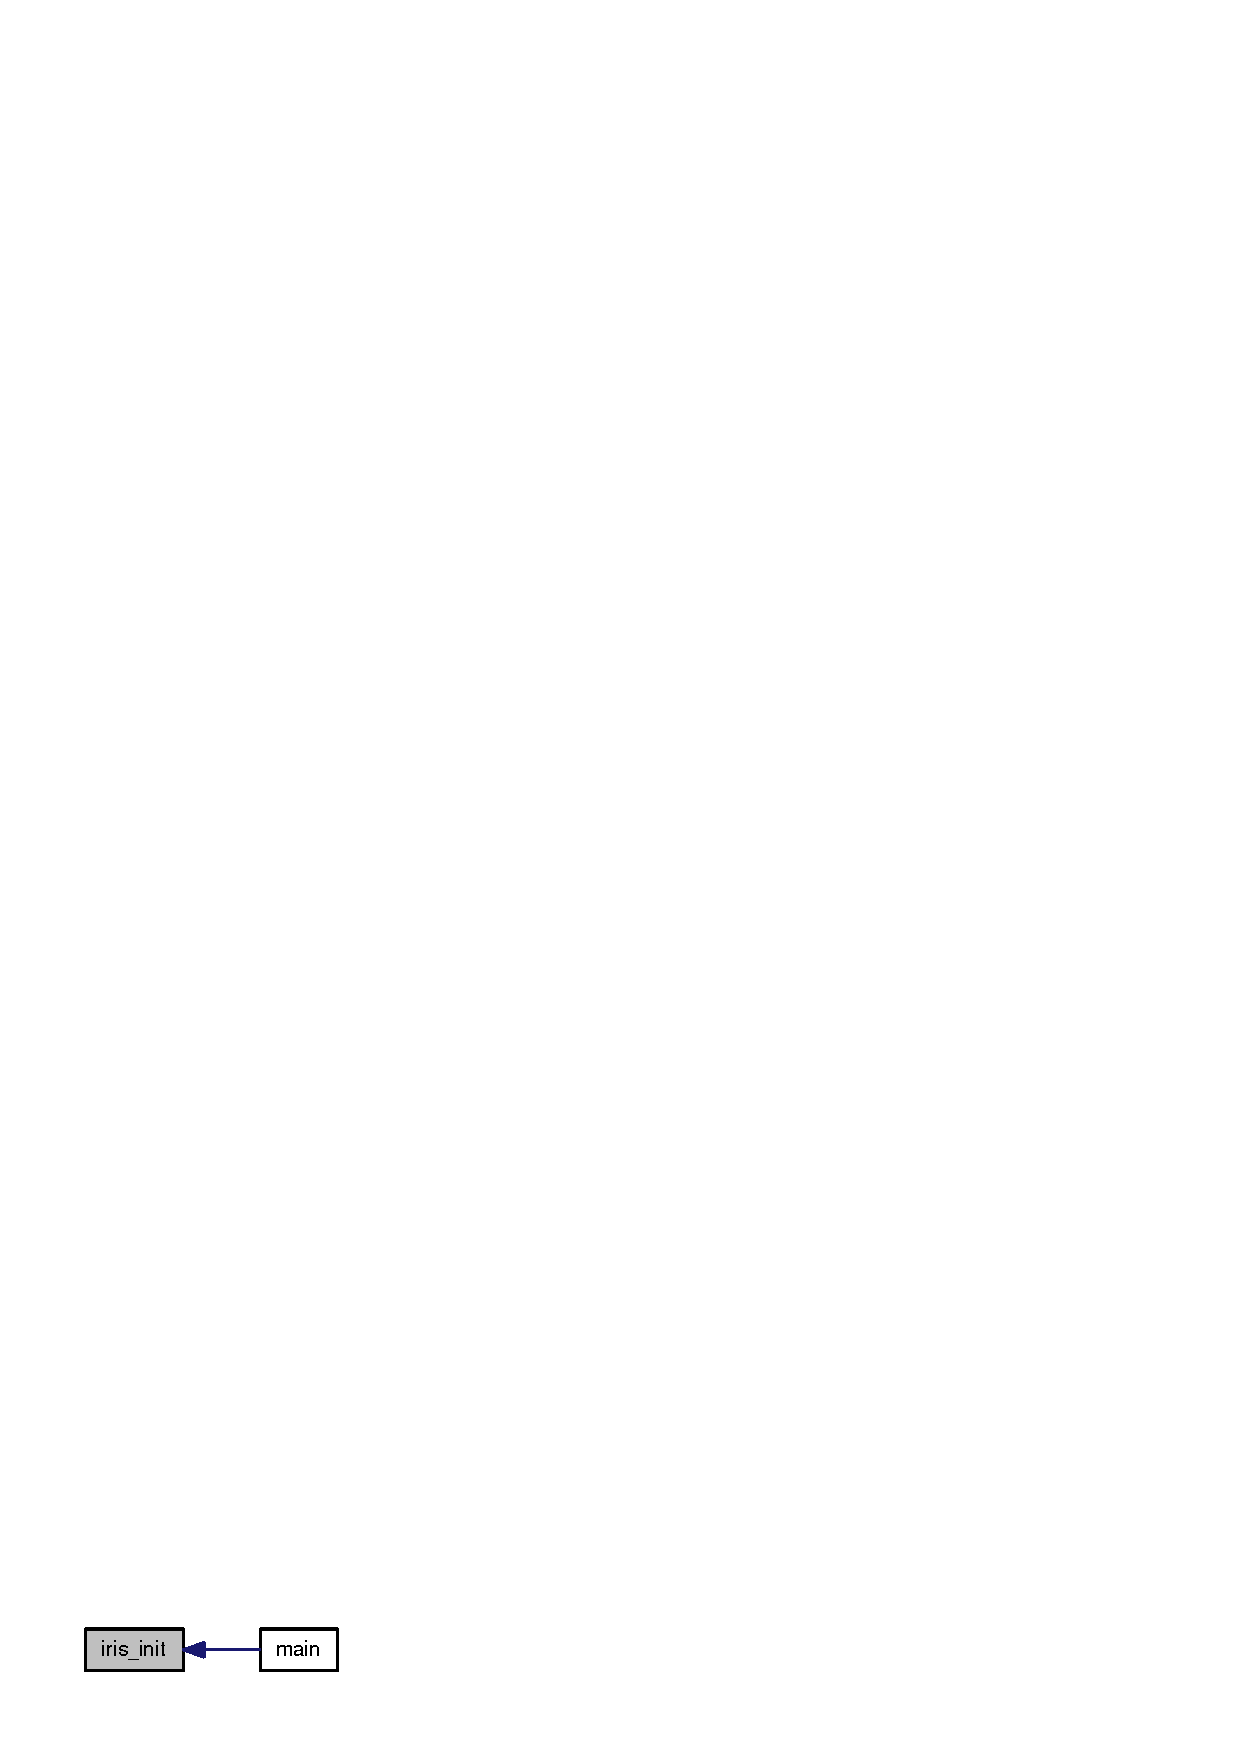
\includegraphics[width=83pt]{manifold__fullsim_8cc_9ceb71c1e1d68963b68464d4bd3aed81_icgraph}
\end{center}
\end{figure}
\index{manifold\_\-fullsim.cc@{manifold\_\-fullsim.cc}!iris\_\-process\_\-options@{iris\_\-process\_\-options}}
\index{iris\_\-process\_\-options@{iris\_\-process\_\-options}!manifold_fullsim.cc@{manifold\_\-fullsim.cc}}
\subsubsection[{iris\_\-process\_\-options}]{\setlength{\rightskip}{0pt plus 5cm}unsigned int iris\_\-process\_\-options (int {\em argc}, \/  char $\ast$ {\em argv}[$\,$])}\label{manifold__fullsim_8cc_d1d4500f982f63302d71d34a7d5381dd}




Definition at line 250 of file manifold\_\-fullsim.cc.

References BANK\_\-BITS, buffer\_\-size, cores\_\-per\_\-node, credits, data, do\_\-two\_\-stage\_\-router, FCFS, grid\_\-size, links, max\_\-phy\_\-link\_\-bits, max\_\-sim\_\-time, MC\_\-ADDR\_\-BITS, mc\_\-positions, msg\_\-type\_\-string, NEGATIVE\_\-FIRST, no\_\-mcs, no\_\-nodes, NORTH\_\-LAST, NORTH\_\-LAST\_\-NON\_\-MINIMAL, ODD\_\-EVEN, ONE\_\-FLIT\_\-REQ, output\_\-path, ports, print\_\-setup, priority\_\-msg\_\-type, PRIORITY\_\-REQ, rc\_\-method, RESPONSE\_\-PKT, ROUND\_\-ROBIN, ROUND\_\-ROBIN\_\-PRIORITY, routing\_\-scheme, sw\_\-arbitration, sw\_\-arbitration\_\-scheme, THREAD\_\-BITS\_\-POSITION, traces, vcs, WEST\_\-FIRST, word, and XY.

Referenced by main().

Here is the caller graph for this function:\nopagebreak
\begin{figure}[H]
\begin{center}
\leavevmode
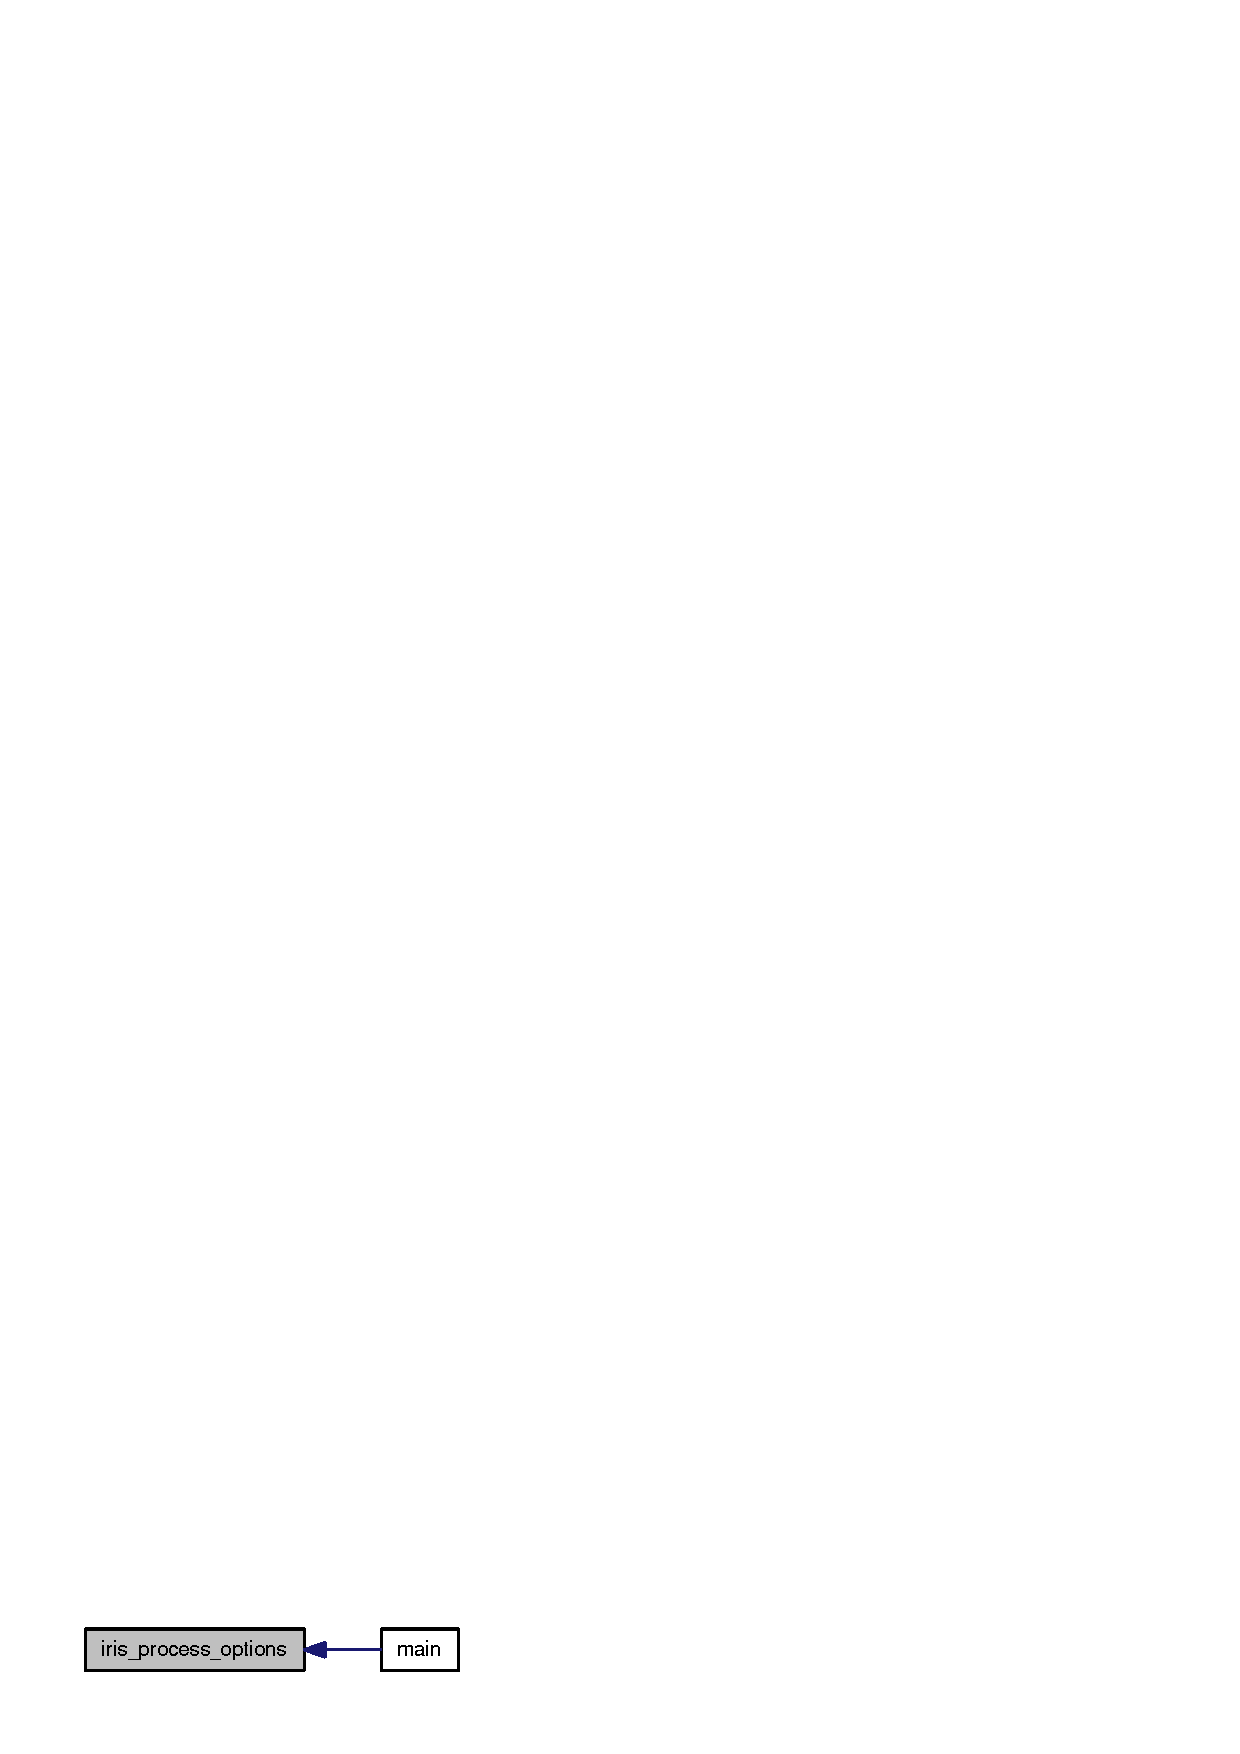
\includegraphics[width=112pt]{manifold__fullsim_8cc_d1d4500f982f63302d71d34a7d5381dd_icgraph}
\end{center}
\end{figure}
\index{manifold\_\-fullsim.cc@{manifold\_\-fullsim.cc}!main@{main}}
\index{main@{main}!manifold_fullsim.cc@{manifold\_\-fullsim.cc}}
\subsubsection[{main}]{\setlength{\rightskip}{0pt plus 5cm}int main (int {\em argc}, \/  char $\ast$ {\em argv}[$\,$])}\label{manifold__fullsim_8cc_0ddf1224851353fc92bfbff6f499fa97}




Definition at line 558 of file manifold\_\-fullsim.cc.

References banner(), cores\_\-per\_\-node, exec\_\-index, exit\_\-code, exit\_\-now(), fatal(), fatal\_\-hook(), help\_\-me, init\_\-quit, iris\_\-init(), iris\_\-process\_\-options(), md\_\-init\_\-decoder(), mysrand(), nice\_\-priority, no\_\-nodes, num\_\-threads, opt\_\-new(), opt\_\-print\_\-options(), opt\_\-process\_\-options(), orphan\_\-fn(), rand\_\-seed, Simulator::Run(), running, signal\_\-exit\_\-now(), signal\_\-sim\_\-stats(), sim\_\-aux\_\-config(), sim\_\-check\_\-options(), sim\_\-exit\_\-buf, sim\_\-main(), sim\_\-post\_\-init(), sim\_\-pre\_\-init(), sim\_\-print\_\-stats(), sim\_\-progfd, sim\_\-progout, sim\_\-reg\_\-options(), sim\_\-reg\_\-stats(), sim\_\-simout, sim\_\-start\_\-time, stat\_\-new(), Simulator::StopAt(), threads, TRUE, usage(), and zesto\_\-component::zesto\_\-component().\index{manifold\_\-fullsim.cc@{manifold\_\-fullsim.cc}!orphan\_\-fn@{orphan\_\-fn}}
\index{orphan\_\-fn@{orphan\_\-fn}!manifold_fullsim.cc@{manifold\_\-fullsim.cc}}
\subsubsection[{orphan\_\-fn}]{\setlength{\rightskip}{0pt plus 5cm}static int orphan\_\-fn (int {\em i}, \/  int {\em argc}, \/  char $\ast$$\ast$ {\em argv})\hspace{0.3cm}{\tt  [static]}}\label{manifold__fullsim_8cc_83995bc1d7a29f4a3f671918e86f8eaa}




Definition at line 121 of file manifold\_\-fullsim.cc.

References exec\_\-index, and FALSE.

Referenced by main().

Here is the caller graph for this function:\nopagebreak
\begin{figure}[H]
\begin{center}
\leavevmode
\includegraphics[width=89pt]{manifold__fullsim_8cc_83995bc1d7a29f4a3f671918e86f8eaa_icgraph}
\end{center}
\end{figure}
\index{manifold\_\-fullsim.cc@{manifold\_\-fullsim.cc}!print\_\-state\_\-at\_\-deadlock@{print\_\-state\_\-at\_\-deadlock}}
\index{print\_\-state\_\-at\_\-deadlock@{print\_\-state\_\-at\_\-deadlock}!manifold_fullsim.cc@{manifold\_\-fullsim.cc}}
\subsubsection[{print\_\-state\_\-at\_\-deadlock}]{\setlength{\rightskip}{0pt plus 5cm}void print\_\-state\_\-at\_\-deadlock (void)}\label{manifold__fullsim_8cc_dd8eeaa0833d2f96796f0ee0f0e98f5c}




Definition at line 154 of file manifold\_\-fullsim.cc.

References no\_\-nodes, and Mesh::routers.\index{manifold\_\-fullsim.cc@{manifold\_\-fullsim.cc}!signal\_\-exit\_\-now@{signal\_\-exit\_\-now}}
\index{signal\_\-exit\_\-now@{signal\_\-exit\_\-now}!manifold_fullsim.cc@{manifold\_\-fullsim.cc}}
\subsubsection[{signal\_\-exit\_\-now}]{\setlength{\rightskip}{0pt plus 5cm}static void signal\_\-exit\_\-now (int {\em sigtype})\hspace{0.3cm}{\tt  [static]}}\label{manifold__fullsim_8cc_eb90a8280771250c1a9ee1d7518cbf63}




Definition at line 70 of file manifold\_\-fullsim.cc.

References sim\_\-exit\_\-now, and TRUE.

Referenced by main().

Here is the caller graph for this function:\nopagebreak
\begin{figure}[H]
\begin{center}
\leavevmode
\includegraphics[width=102pt]{manifold__fullsim_8cc_eb90a8280771250c1a9ee1d7518cbf63_icgraph}
\end{center}
\end{figure}
\index{manifold\_\-fullsim.cc@{manifold\_\-fullsim.cc}!signal\_\-sim\_\-stats@{signal\_\-sim\_\-stats}}
\index{signal\_\-sim\_\-stats@{signal\_\-sim\_\-stats}!manifold_fullsim.cc@{manifold\_\-fullsim.cc}}
\subsubsection[{signal\_\-sim\_\-stats}]{\setlength{\rightskip}{0pt plus 5cm}static void signal\_\-sim\_\-stats (int {\em sigtype})\hspace{0.3cm}{\tt  [static]}}\label{manifold__fullsim_8cc_206bcb38d2bf43a4c9e8e82d038f1643}




Definition at line 63 of file manifold\_\-fullsim.cc.

References sim\_\-dump\_\-stats, and TRUE.

Referenced by main().

Here is the caller graph for this function:\nopagebreak
\begin{figure}[H]
\begin{center}
\leavevmode
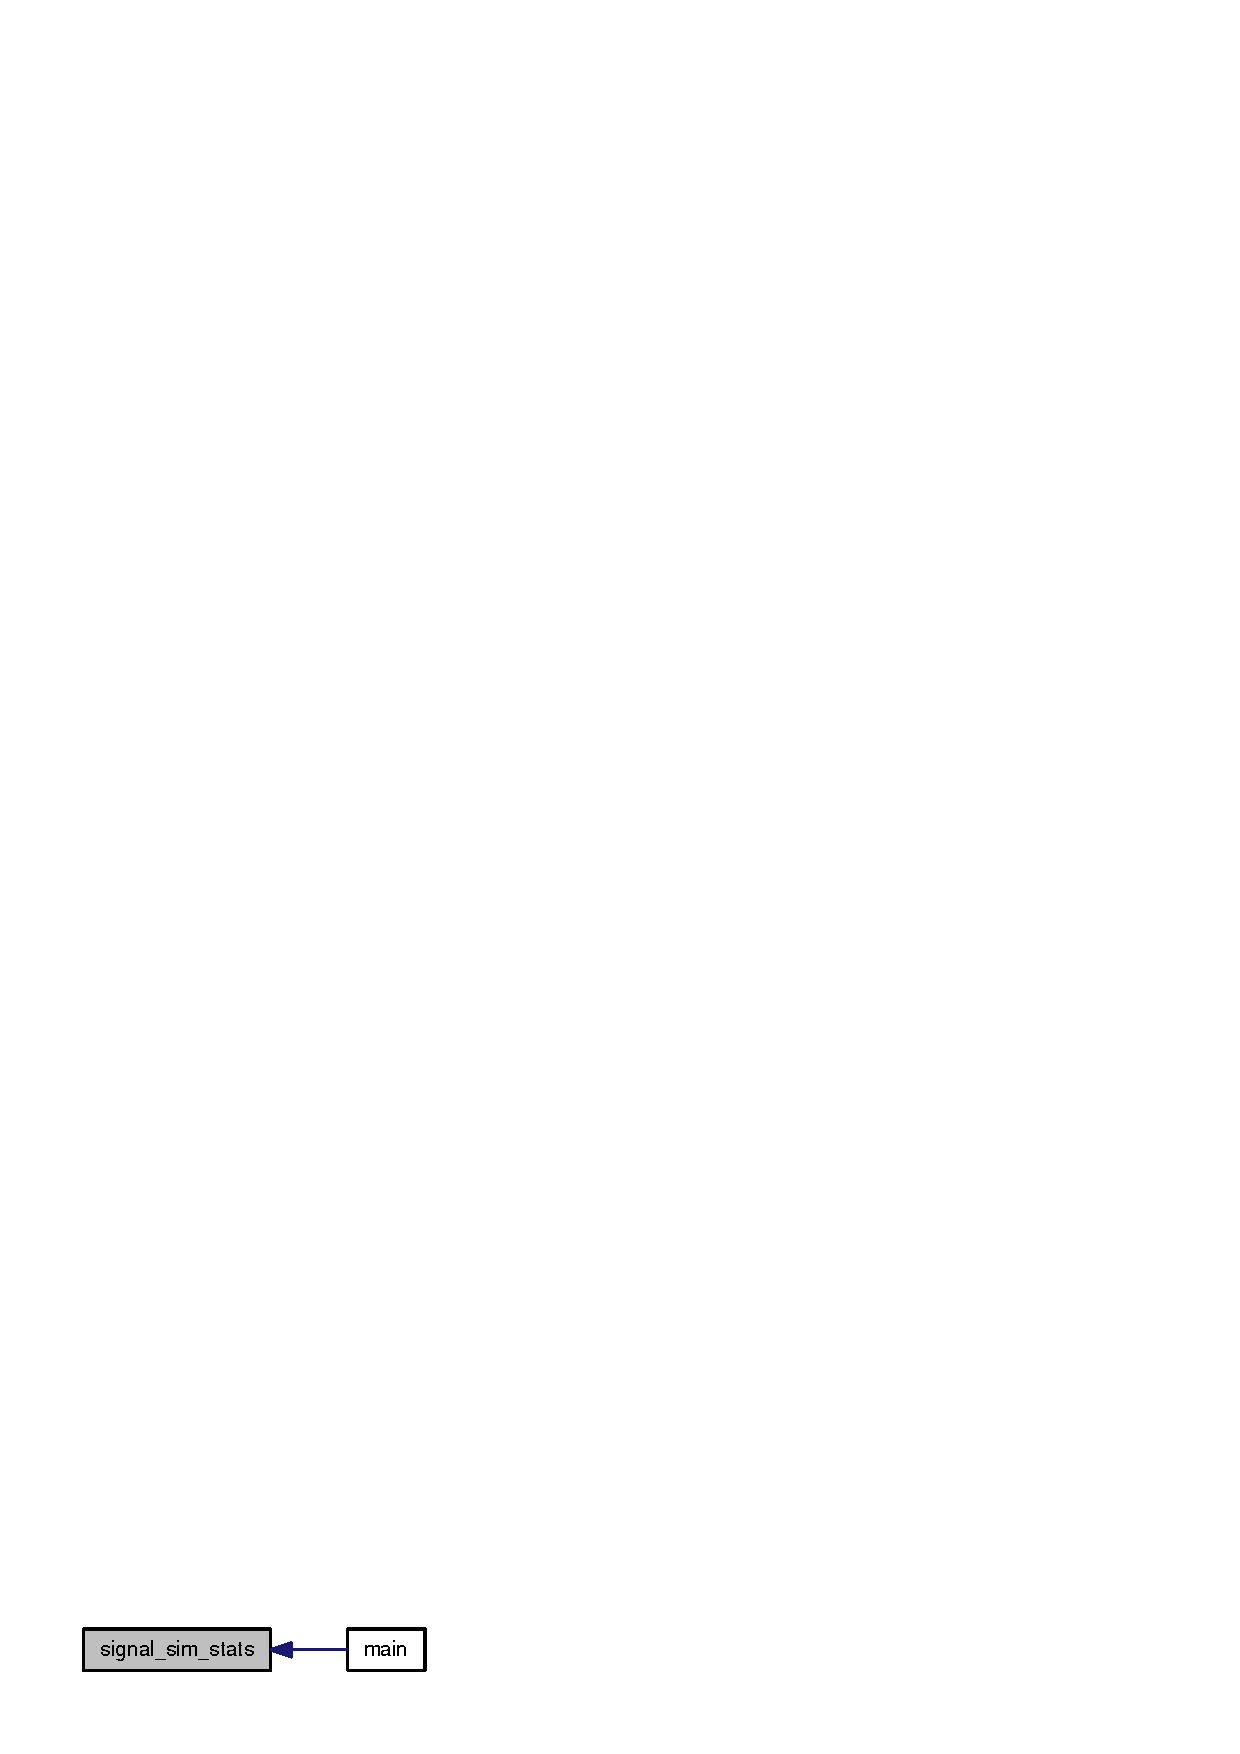
\includegraphics[width=104pt]{manifold__fullsim_8cc_206bcb38d2bf43a4c9e8e82d038f1643_icgraph}
\end{center}
\end{figure}
\index{manifold\_\-fullsim.cc@{manifold\_\-fullsim.cc}!sim\_\-print\_\-stats@{sim\_\-print\_\-stats}}
\index{sim\_\-print\_\-stats@{sim\_\-print\_\-stats}!manifold_fullsim.cc@{manifold\_\-fullsim.cc}}
\subsubsection[{sim\_\-print\_\-stats}]{\setlength{\rightskip}{0pt plus 5cm}void sim\_\-print\_\-stats (FILE $\ast$ {\em fd})}\label{manifold__fullsim_8cc_ebded8bcfea50ac2770a680b87509424}




Definition at line 164 of file manifold\_\-fullsim.cc.

References Mesh::interfaces, Mesh::link\_\-a, Mesh::link\_\-b, links, MAX, max\_\-phy\_\-link\_\-bits, max\_\-sim\_\-time, no\_\-nodes, running, sim\_\-aux\_\-stats(), sim\_\-elapsed\_\-time, sim\_\-end\_\-time, and sim\_\-start\_\-time.

Referenced by exit\_\-now(), and main().

Here is the caller graph for this function:\nopagebreak
\begin{figure}[H]
\begin{center}
\leavevmode
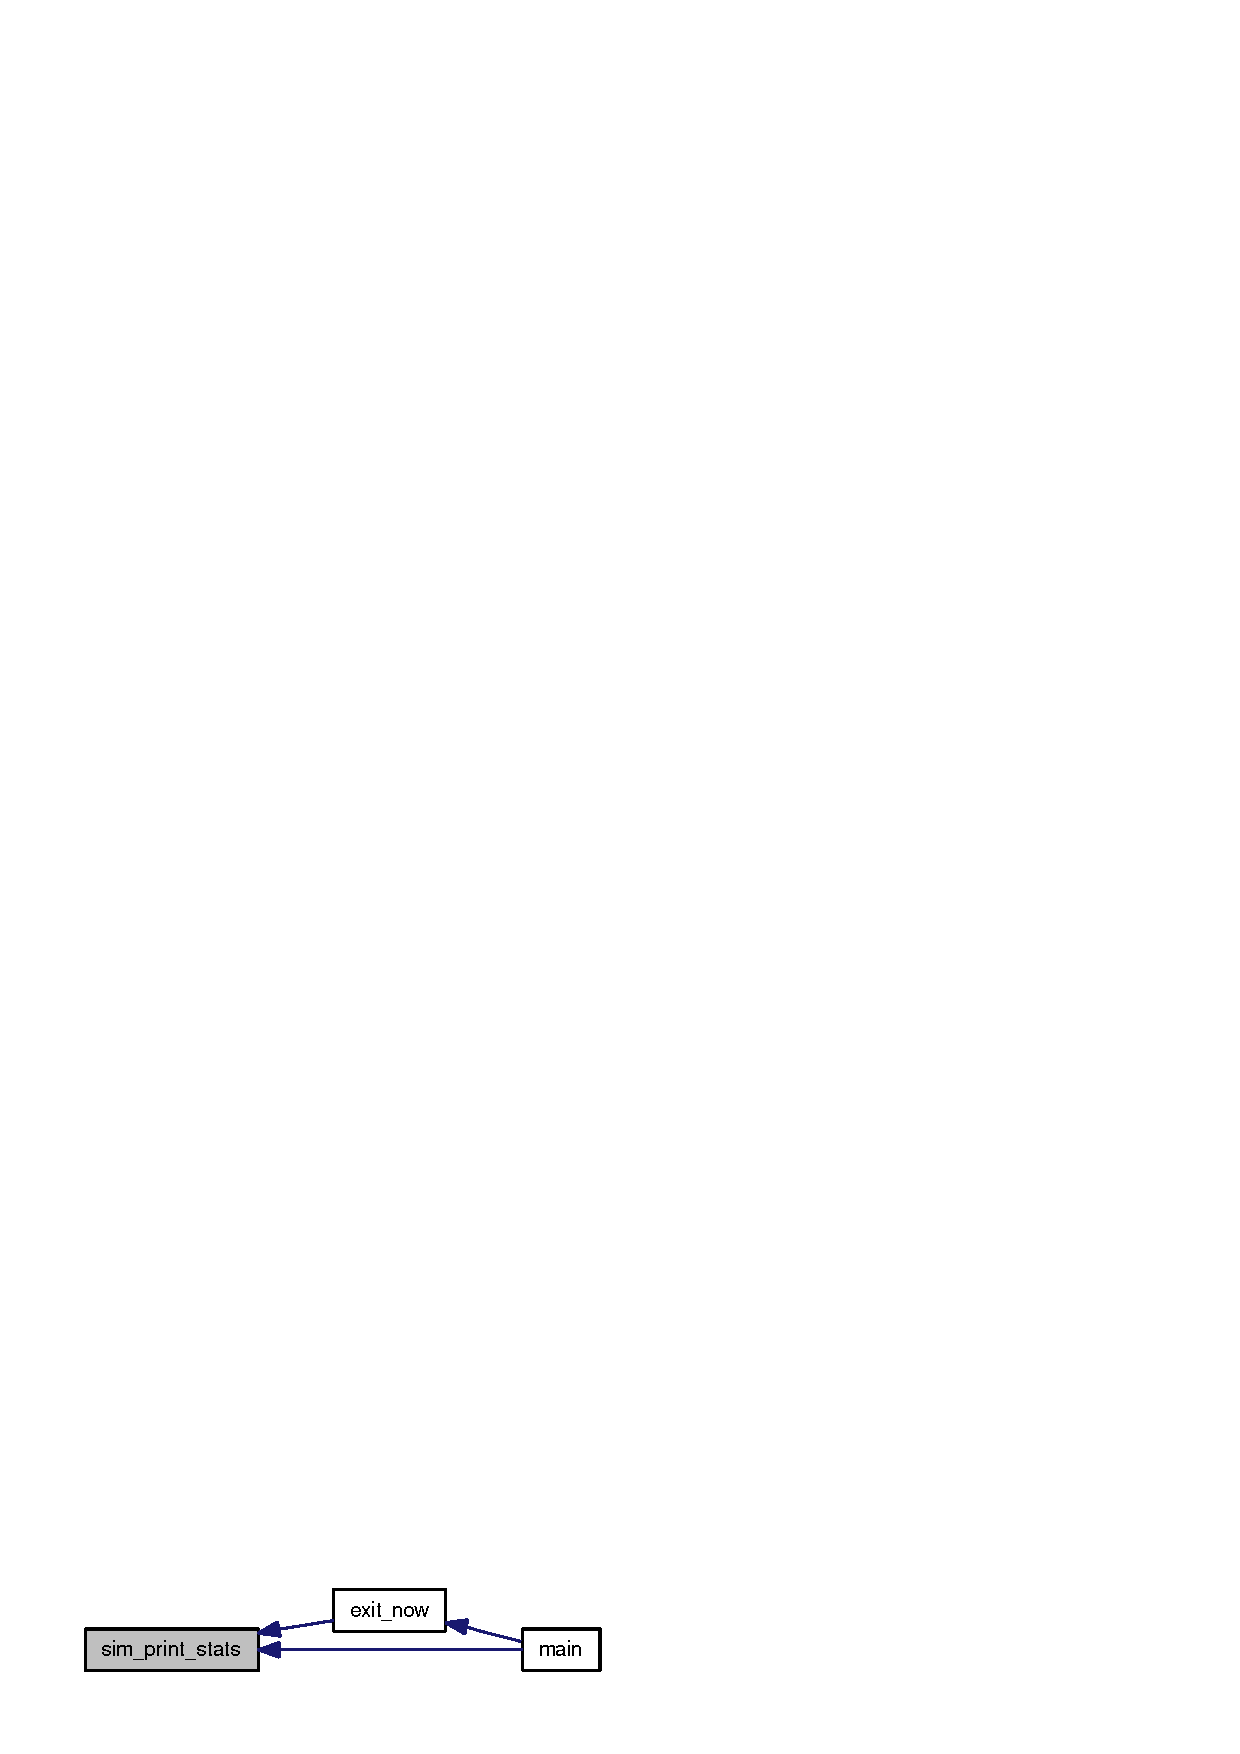
\includegraphics[width=146pt]{manifold__fullsim_8cc_ebded8bcfea50ac2770a680b87509424_icgraph}
\end{center}
\end{figure}
\index{manifold\_\-fullsim.cc@{manifold\_\-fullsim.cc}!usage@{usage}}
\index{usage@{usage}!manifold_fullsim.cc@{manifold\_\-fullsim.cc}}
\subsubsection[{usage}]{\setlength{\rightskip}{0pt plus 5cm}static void usage (FILE $\ast$ {\em fd}, \/  int {\em argc}, \/  char $\ast$$\ast$ {\em argv})\hspace{0.3cm}{\tt  [static]}}\label{manifold__fullsim_8cc_4b40663cf65d8f5b9ef33ac7cdad3ea2}




Definition at line 144 of file manifold\_\-fullsim.cc.

References opt\_\-print\_\-help().

Referenced by main().

Here is the caller graph for this function:\nopagebreak
\begin{figure}[H]
\begin{center}
\leavevmode
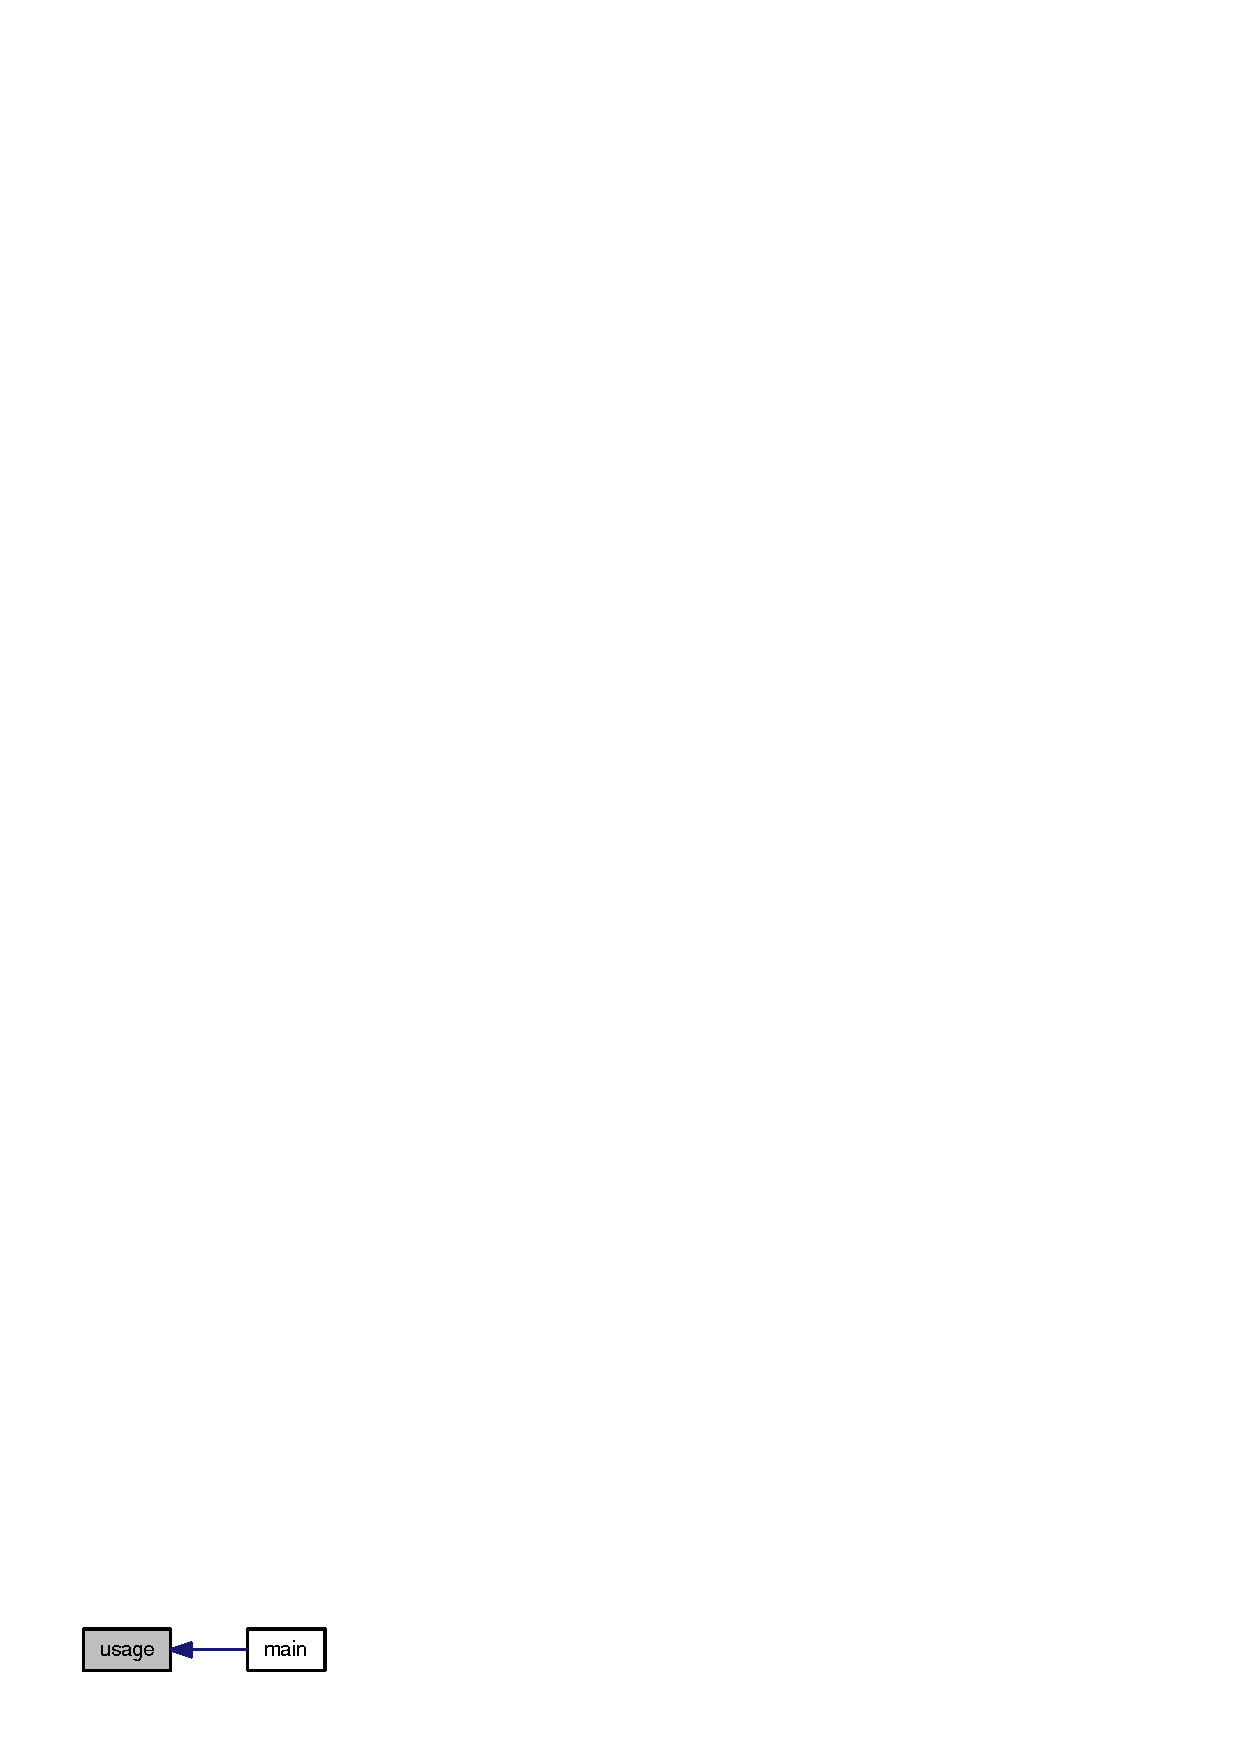
\includegraphics[width=80pt]{manifold__fullsim_8cc_4b40663cf65d8f5b9ef33ac7cdad3ea2_icgraph}
\end{center}
\end{figure}


\subsection{Variable Documentation}
\index{manifold\_\-fullsim.cc@{manifold\_\-fullsim.cc}!cores\_\-per\_\-node@{cores\_\-per\_\-node}}
\index{cores\_\-per\_\-node@{cores\_\-per\_\-node}!manifold_fullsim.cc@{manifold\_\-fullsim.cc}}
\subsubsection[{cores\_\-per\_\-node}]{\setlength{\rightskip}{0pt plus 5cm}unsigned int {\bf cores\_\-per\_\-node} = 1}\label{manifold__fullsim_8cc_d1fe1c89980f30a3204e89fe23449677}




Definition at line 48 of file manifold\_\-fullsim.cc.

Referenced by iris\_\-process\_\-options(), main(), sim\_\-post\_\-init(), and uncore\_\-t::uncore\_\-t().\index{manifold\_\-fullsim.cc@{manifold\_\-fullsim.cc}!data@{data}}
\index{data@{data}!manifold_fullsim.cc@{manifold\_\-fullsim.cc}}
\subsubsection[{data}]{\setlength{\rightskip}{0pt plus 5cm}string {\bf data}}\label{manifold__fullsim_8cc_bbd74d905a52bdcb0b21f0b8b4fcc1ba}




Definition at line 47 of file manifold\_\-fullsim.cc.

Referenced by GenericRouterVct::do\_\-switch\_\-traversal(), GenericRouterVcs::do\_\-switch\_\-traversal(), GenericRouterNoVcs::do\_\-switch\_\-traversal(), GenericRouterAdaptive::do\_\-switch\_\-traversal(), GenericRouterVct::handle\_\-link\_\-arrival\_\-event(), GenericRouterVcs::handle\_\-link\_\-arrival\_\-event(), GenericRouterNoVcs::handle\_\-link\_\-arrival\_\-event(), GenericLink::handle\_\-link\_\-arrival\_\-event(), GenericRouterAdaptive::handle\_\-link\_\-arrival\_\-event\_\-multiple\_\-flit\_\-in\_\-buffer(), GenericRouterAdaptive::handle\_\-link\_\-arrival\_\-event\_\-one\_\-msg\_\-per\_\-buffer(), iris\_\-process\_\-options(), main(), HeadFlit::populate\_\-head\_\-flit(), TailFlit::populate\_\-tail\_\-flit(), GenericRouterVct::send\_\-credit\_\-back(), GenericRouterVcs::send\_\-credit\_\-back(), GenericRouterNoVcs::send\_\-credit\_\-back(), and GenericRouterAdaptive::send\_\-credit\_\-back().\index{manifold\_\-fullsim.cc@{manifold\_\-fullsim.cc}!exec\_\-index@{exec\_\-index}}
\index{exec\_\-index@{exec\_\-index}!manifold_fullsim.cc@{manifold\_\-fullsim.cc}}
\subsubsection[{exec\_\-index}]{\setlength{\rightskip}{0pt plus 5cm}int {\bf exec\_\-index} = -1\hspace{0.3cm}{\tt  [static]}}\label{manifold__fullsim_8cc_4afde0d7feaebf12b1542f128c65042a}




Definition at line 105 of file manifold\_\-fullsim.cc.

Referenced by main(), and orphan\_\-fn().\index{manifold\_\-fullsim.cc@{manifold\_\-fullsim.cc}!exit\_\-code@{exit\_\-code}}
\index{exit\_\-code@{exit\_\-code}!manifold_fullsim.cc@{manifold\_\-fullsim.cc}}
\subsubsection[{exit\_\-code}]{\setlength{\rightskip}{0pt plus 5cm}int {\bf exit\_\-code}}\label{manifold__fullsim_8cc_b1729158be557ef60548f7b7575ea4dd}




Definition at line 59 of file manifold\_\-fullsim.cc.

Referenced by main().\index{manifold\_\-fullsim.cc@{manifold\_\-fullsim.cc}!help\_\-me@{help\_\-me}}
\index{help\_\-me@{help\_\-me}!manifold_fullsim.cc@{manifold\_\-fullsim.cc}}
\subsubsection[{help\_\-me}]{\setlength{\rightskip}{0pt plus 5cm}bool {\bf help\_\-me}}\label{manifold__fullsim_8cc_98b74f22826e26c7727ce84f6d3a621b}




Definition at line 108 of file manifold\_\-fullsim.cc.

Referenced by main().\index{manifold\_\-fullsim.cc@{manifold\_\-fullsim.cc}!init\_\-quit@{init\_\-quit}}
\index{init\_\-quit@{init\_\-quit}!manifold_fullsim.cc@{manifold\_\-fullsim.cc}}
\subsubsection[{init\_\-quit}]{\setlength{\rightskip}{0pt plus 5cm}bool {\bf init\_\-quit}}\label{manifold__fullsim_8cc_1d93ba7fce2ae0edcb3665632a12bd49}




Definition at line 114 of file manifold\_\-fullsim.cc.

Referenced by main().\index{manifold\_\-fullsim.cc@{manifold\_\-fullsim.cc}!mesh@{mesh}}
\index{mesh@{mesh}!manifold_fullsim.cc@{manifold\_\-fullsim.cc}}
\subsubsection[{mesh}]{\setlength{\rightskip}{0pt plus 5cm}{\bf Mesh}$\ast$ {\bf mesh}}\label{manifold__fullsim_8cc_6e08f89b32254fb4b129720418e7c6ea}




Definition at line 55 of file manifold\_\-fullsim.cc.\index{manifold\_\-fullsim.cc@{manifold\_\-fullsim.cc}!nice\_\-priority@{nice\_\-priority}}
\index{nice\_\-priority@{nice\_\-priority}!manifold_fullsim.cc@{manifold\_\-fullsim.cc}}
\subsubsection[{nice\_\-priority}]{\setlength{\rightskip}{0pt plus 5cm}int {\bf nice\_\-priority}}\label{manifold__fullsim_8cc_1cb688b2b9eda644e545e25f039761e4}




Definition at line 117 of file manifold\_\-fullsim.cc.

Referenced by main().\index{manifold\_\-fullsim.cc@{manifold\_\-fullsim.cc}!rand\_\-seed@{rand\_\-seed}}
\index{rand\_\-seed@{rand\_\-seed}!manifold_fullsim.cc@{manifold\_\-fullsim.cc}}
\subsubsection[{rand\_\-seed}]{\setlength{\rightskip}{0pt plus 5cm}int {\bf rand\_\-seed}}\label{manifold__fullsim_8cc_b58df36fd429cab6ab2f2dedd531f7a9}




Definition at line 111 of file manifold\_\-fullsim.cc.

Referenced by main().\index{manifold\_\-fullsim.cc@{manifold\_\-fullsim.cc}!running@{running}}
\index{running@{running}!manifold_fullsim.cc@{manifold\_\-fullsim.cc}}
\subsubsection[{running}]{\setlength{\rightskip}{0pt plus 5cm}int {\bf running} = FALSE\hspace{0.3cm}{\tt  [static]}}\label{manifold__fullsim_8cc_2f45113638a0b749a8a205d2cd7fb42b}




Definition at line 150 of file manifold\_\-fullsim.cc.

Referenced by main(), and sim\_\-print\_\-stats().\index{manifold\_\-fullsim.cc@{manifold\_\-fullsim.cc}!s@{s}}
\index{s@{s}!manifold_fullsim.cc@{manifold\_\-fullsim.cc}}
\subsubsection[{s}]{\setlength{\rightskip}{0pt plus 5cm}char$\ast$ {\bf s}}\label{manifold__fullsim_8cc_b51cd24d34f6509eafb5e059f4c7d10e}




Definition at line 58 of file manifold\_\-fullsim.cc.

Referenced by banner().\index{manifold\_\-fullsim.cc@{manifold\_\-fullsim.cc}!sim\_\-dump\_\-stats@{sim\_\-dump\_\-stats}}
\index{sim\_\-dump\_\-stats@{sim\_\-dump\_\-stats}!manifold_fullsim.cc@{manifold\_\-fullsim.cc}}
\subsubsection[{sim\_\-dump\_\-stats}]{\setlength{\rightskip}{0pt plus 5cm}int {\bf sim\_\-dump\_\-stats} = FALSE}\label{manifold__fullsim_8cc_5f0267e6bed91a9151ebcc5e0a7557dc}




Definition at line 91 of file manifold\_\-fullsim.cc.

Referenced by signal\_\-sim\_\-stats().\index{manifold\_\-fullsim.cc@{manifold\_\-fullsim.cc}!sim\_\-elapsed\_\-time@{sim\_\-elapsed\_\-time}}
\index{sim\_\-elapsed\_\-time@{sim\_\-elapsed\_\-time}!manifold_fullsim.cc@{manifold\_\-fullsim.cc}}
\subsubsection[{sim\_\-elapsed\_\-time}]{\setlength{\rightskip}{0pt plus 5cm}int {\bf sim\_\-elapsed\_\-time}}\label{manifold__fullsim_8cc_84462569a8ea1951d2547b98eaa30f25}




Definition at line 78 of file manifold\_\-fullsim.cc.

Referenced by sim\_\-print\_\-stats().\index{manifold\_\-fullsim.cc@{manifold\_\-fullsim.cc}!sim\_\-end\_\-time@{sim\_\-end\_\-time}}
\index{sim\_\-end\_\-time@{sim\_\-end\_\-time}!manifold_fullsim.cc@{manifold\_\-fullsim.cc}}
\subsubsection[{sim\_\-end\_\-time}]{\setlength{\rightskip}{0pt plus 5cm}time\_\-t {\bf sim\_\-end\_\-time}}\label{manifold__fullsim_8cc_5db757faa4910d3f30bfddc7c81261e8}




Definition at line 77 of file manifold\_\-fullsim.cc.

Referenced by sim\_\-print\_\-stats().\index{manifold\_\-fullsim.cc@{manifold\_\-fullsim.cc}!sim\_\-exit\_\-buf@{sim\_\-exit\_\-buf}}
\index{sim\_\-exit\_\-buf@{sim\_\-exit\_\-buf}!manifold_fullsim.cc@{manifold\_\-fullsim.cc}}
\subsubsection[{sim\_\-exit\_\-buf}]{\setlength{\rightskip}{0pt plus 5cm}jmp\_\-buf {\bf sim\_\-exit\_\-buf}}\label{manifold__fullsim_8cc_84727c65b24d2e32fd3d4a7af53aa15a}




Definition at line 88 of file manifold\_\-fullsim.cc.

Referenced by main(), md\_\-fetch\_\-inst(), core\_\-commit\_\-STM\_\-t::step(), and core\_\-commit\_\-DPM\_\-t::step().\index{manifold\_\-fullsim.cc@{manifold\_\-fullsim.cc}!sim\_\-exit\_\-now@{sim\_\-exit\_\-now}}
\index{sim\_\-exit\_\-now@{sim\_\-exit\_\-now}!manifold_fullsim.cc@{manifold\_\-fullsim.cc}}
\subsubsection[{sim\_\-exit\_\-now}]{\setlength{\rightskip}{0pt plus 5cm}int {\bf sim\_\-exit\_\-now} = FALSE}\label{manifold__fullsim_8cc_e6c582e7e1a51970f03ee0c8bb8776df}




Definition at line 85 of file manifold\_\-fullsim.cc.

Referenced by signal\_\-exit\_\-now().\index{manifold\_\-fullsim.cc@{manifold\_\-fullsim.cc}!sim\_\-odb@{sim\_\-odb}}
\index{sim\_\-odb@{sim\_\-odb}!manifold_fullsim.cc@{manifold\_\-fullsim.cc}}
\subsubsection[{sim\_\-odb}]{\setlength{\rightskip}{0pt plus 5cm}struct {\bf opt\_\-odb\_\-t}$\ast$ {\bf sim\_\-odb}}\label{manifold__fullsim_8cc_5520d419f4ed203a8f4496330bef06e3}




Definition at line 94 of file manifold\_\-fullsim.cc.\index{manifold\_\-fullsim.cc@{manifold\_\-fullsim.cc}!sim\_\-progfd@{sim\_\-progfd}}
\index{sim\_\-progfd@{sim\_\-progfd}!manifold_fullsim.cc@{manifold\_\-fullsim.cc}}
\subsubsection[{sim\_\-progfd}]{\setlength{\rightskip}{0pt plus 5cm}FILE$\ast$ {\bf sim\_\-progfd} = NULL}\label{manifold__fullsim_8cc_f93f90c77918d1b430318725f0f607a8}




Definition at line 102 of file manifold\_\-fullsim.cc.

Referenced by main().\index{manifold\_\-fullsim.cc@{manifold\_\-fullsim.cc}!sim\_\-progout@{sim\_\-progout}}
\index{sim\_\-progout@{sim\_\-progout}!manifold_fullsim.cc@{manifold\_\-fullsim.cc}}
\subsubsection[{sim\_\-progout}]{\setlength{\rightskip}{0pt plus 5cm}char$\ast$ {\bf sim\_\-progout} = NULL}\label{manifold__fullsim_8cc_21fe317600267fa77e054df4355779dc}




Definition at line 101 of file manifold\_\-fullsim.cc.

Referenced by main().\index{manifold\_\-fullsim.cc@{manifold\_\-fullsim.cc}!sim\_\-sdb@{sim\_\-sdb}}
\index{sim\_\-sdb@{sim\_\-sdb}!manifold_fullsim.cc@{manifold\_\-fullsim.cc}}
\subsubsection[{sim\_\-sdb}]{\setlength{\rightskip}{0pt plus 5cm}struct {\bf stat\_\-sdb\_\-t}$\ast$ {\bf sim\_\-sdb}}\label{manifold__fullsim_8cc_2f46df2af0ce568e5ae2ea2a78cb006b}




Definition at line 97 of file manifold\_\-fullsim.cc.\index{manifold\_\-fullsim.cc@{manifold\_\-fullsim.cc}!sim\_\-simout@{sim\_\-simout}}
\index{sim\_\-simout@{sim\_\-simout}!manifold_fullsim.cc@{manifold\_\-fullsim.cc}}
\subsubsection[{sim\_\-simout}]{\setlength{\rightskip}{0pt plus 5cm}char$\ast$ {\bf sim\_\-simout} = NULL}\label{manifold__fullsim_8cc_09cbb844712d19de24f7ec8a414d4266}




Definition at line 100 of file manifold\_\-fullsim.cc.

Referenced by main().\index{manifold\_\-fullsim.cc@{manifold\_\-fullsim.cc}!sim\_\-start\_\-time@{sim\_\-start\_\-time}}
\index{sim\_\-start\_\-time@{sim\_\-start\_\-time}!manifold_fullsim.cc@{manifold\_\-fullsim.cc}}
\subsubsection[{sim\_\-start\_\-time}]{\setlength{\rightskip}{0pt plus 5cm}time\_\-t {\bf sim\_\-start\_\-time}}\label{manifold__fullsim_8cc_e8d0794b6bec1dfbd28ca90a7a08d2b4}




Definition at line 76 of file manifold\_\-fullsim.cc.

Referenced by main(), sim\_\-main(), and sim\_\-print\_\-stats().\index{manifold\_\-fullsim.cc@{manifold\_\-fullsim.cc}!sim\_\-swap\_\-bytes@{sim\_\-swap\_\-bytes}}
\index{sim\_\-swap\_\-bytes@{sim\_\-swap\_\-bytes}!manifold_fullsim.cc@{manifold\_\-fullsim.cc}}
\subsubsection[{sim\_\-swap\_\-bytes}]{\setlength{\rightskip}{0pt plus 5cm}int {\bf sim\_\-swap\_\-bytes}}\label{manifold__fullsim_8cc_feede3aab9267fb42b819ad7bc47247a}




Definition at line 81 of file manifold\_\-fullsim.cc.\index{manifold\_\-fullsim.cc@{manifold\_\-fullsim.cc}!sim\_\-swap\_\-words@{sim\_\-swap\_\-words}}
\index{sim\_\-swap\_\-words@{sim\_\-swap\_\-words}!manifold_fullsim.cc@{manifold\_\-fullsim.cc}}
\subsubsection[{sim\_\-swap\_\-words}]{\setlength{\rightskip}{0pt plus 5cm}int {\bf sim\_\-swap\_\-words}}\label{manifold__fullsim_8cc_a1267d1f1ee712bf4d37a9f7c4d2e913}




Definition at line 82 of file manifold\_\-fullsim.cc.\index{manifold\_\-fullsim.cc@{manifold\_\-fullsim.cc}!word@{word}}
\index{word@{word}!manifold_fullsim.cc@{manifold\_\-fullsim.cc}}
\subsubsection[{word}]{\setlength{\rightskip}{0pt plus 5cm}string {\bf word}}\label{manifold__fullsim_8cc_6e1612f2124fda0de95b60c68c23949a}




Definition at line 47 of file manifold\_\-fullsim.cc.

Referenced by iris\_\-process\_\-options(), and main().